\documentclass[12pt, a4paper]{article}

\usepackage{ctex}
\usepackage{float, booktabs, parskip}
\usepackage{amsmath, amsthm, amssymb, mathrsfs, bm}
\usepackage{graphicx, subfigure, svg}
\usepackage{hyperref, endnotes}
\usepackage{listings}

\setlength{\parindent}{4em}
\setlength{\parskip}{1em}
\allowdisplaybreaks[4]


\newcommand{\di}{{\mathrm{d}}}


\title{{\Huge{\textbf{Homework 3 \\}}}}
\author{刘滨瑞 \quad 2021012579 \quad 未央-水木12}

\begin{document}

\maketitle

    \section{}

        \begin{enumerate}
        \item 从缓坡过渡到陡坡。从上游（缓流）到下游（急流），过临界水深。
        \item 从陡坡过渡到陡坡。从上游（急流）到下游（急流）。控制水深在上游。
        \item 从缓坡过渡到缓坡。从上游（缓流）到下游（缓流）。控制水深在下游。
        \item 从陡坡过渡到缓坡。从上游（急流）到下游（缓流）。发生水跃。
        \end{enumerate}

        据此绘制的水面曲线参见图1。

        \begin{figure}[htbp]
        \centering
        \subfigure[(1)水面曲线]{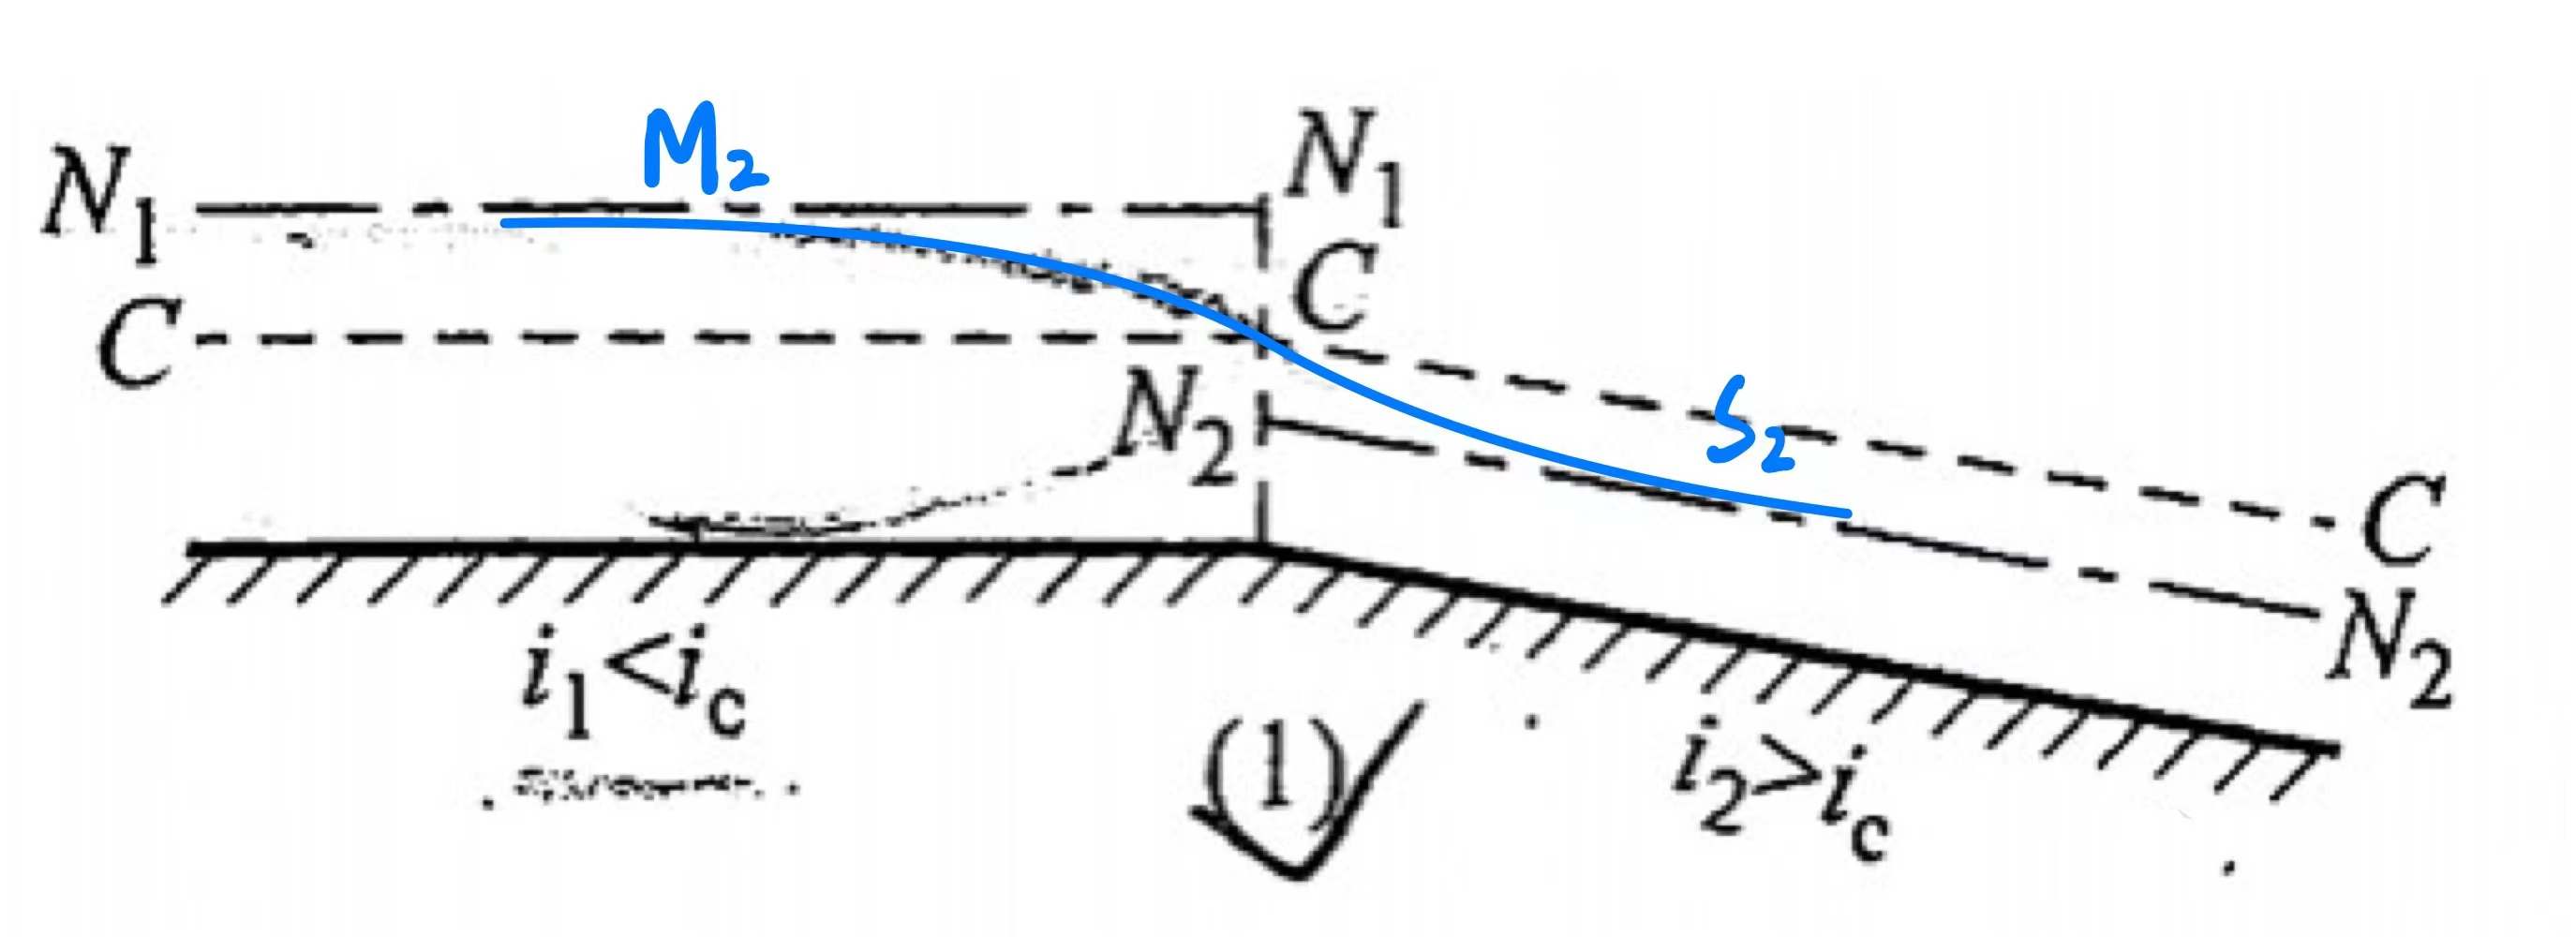
\includegraphics[width=0.80\textwidth]{./assets/1-1.jpg}}
        \subfigure[(2)水面曲线]{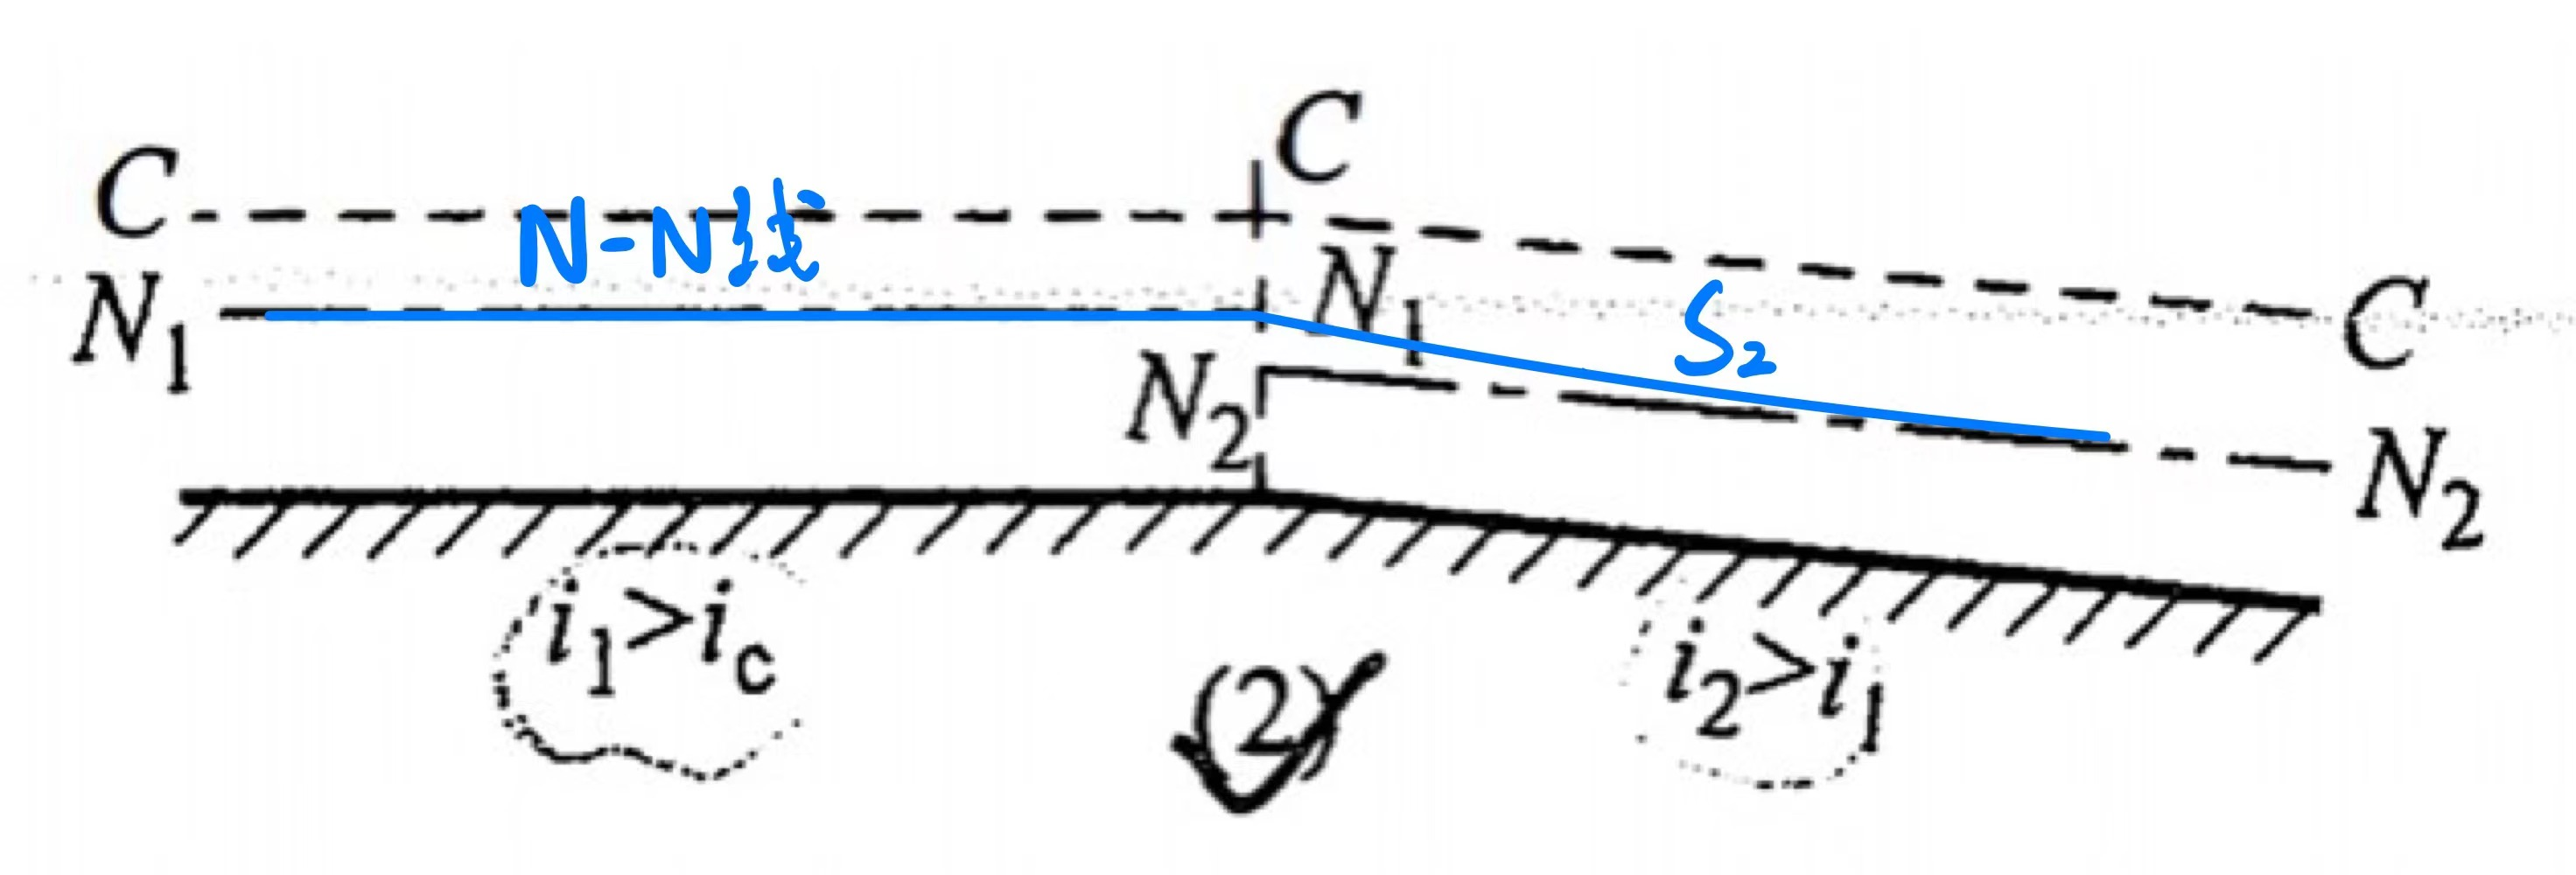
\includegraphics[width=0.80\textwidth]{./assets/1-2.jpg}}
        \subfigure[(3)水面曲线]{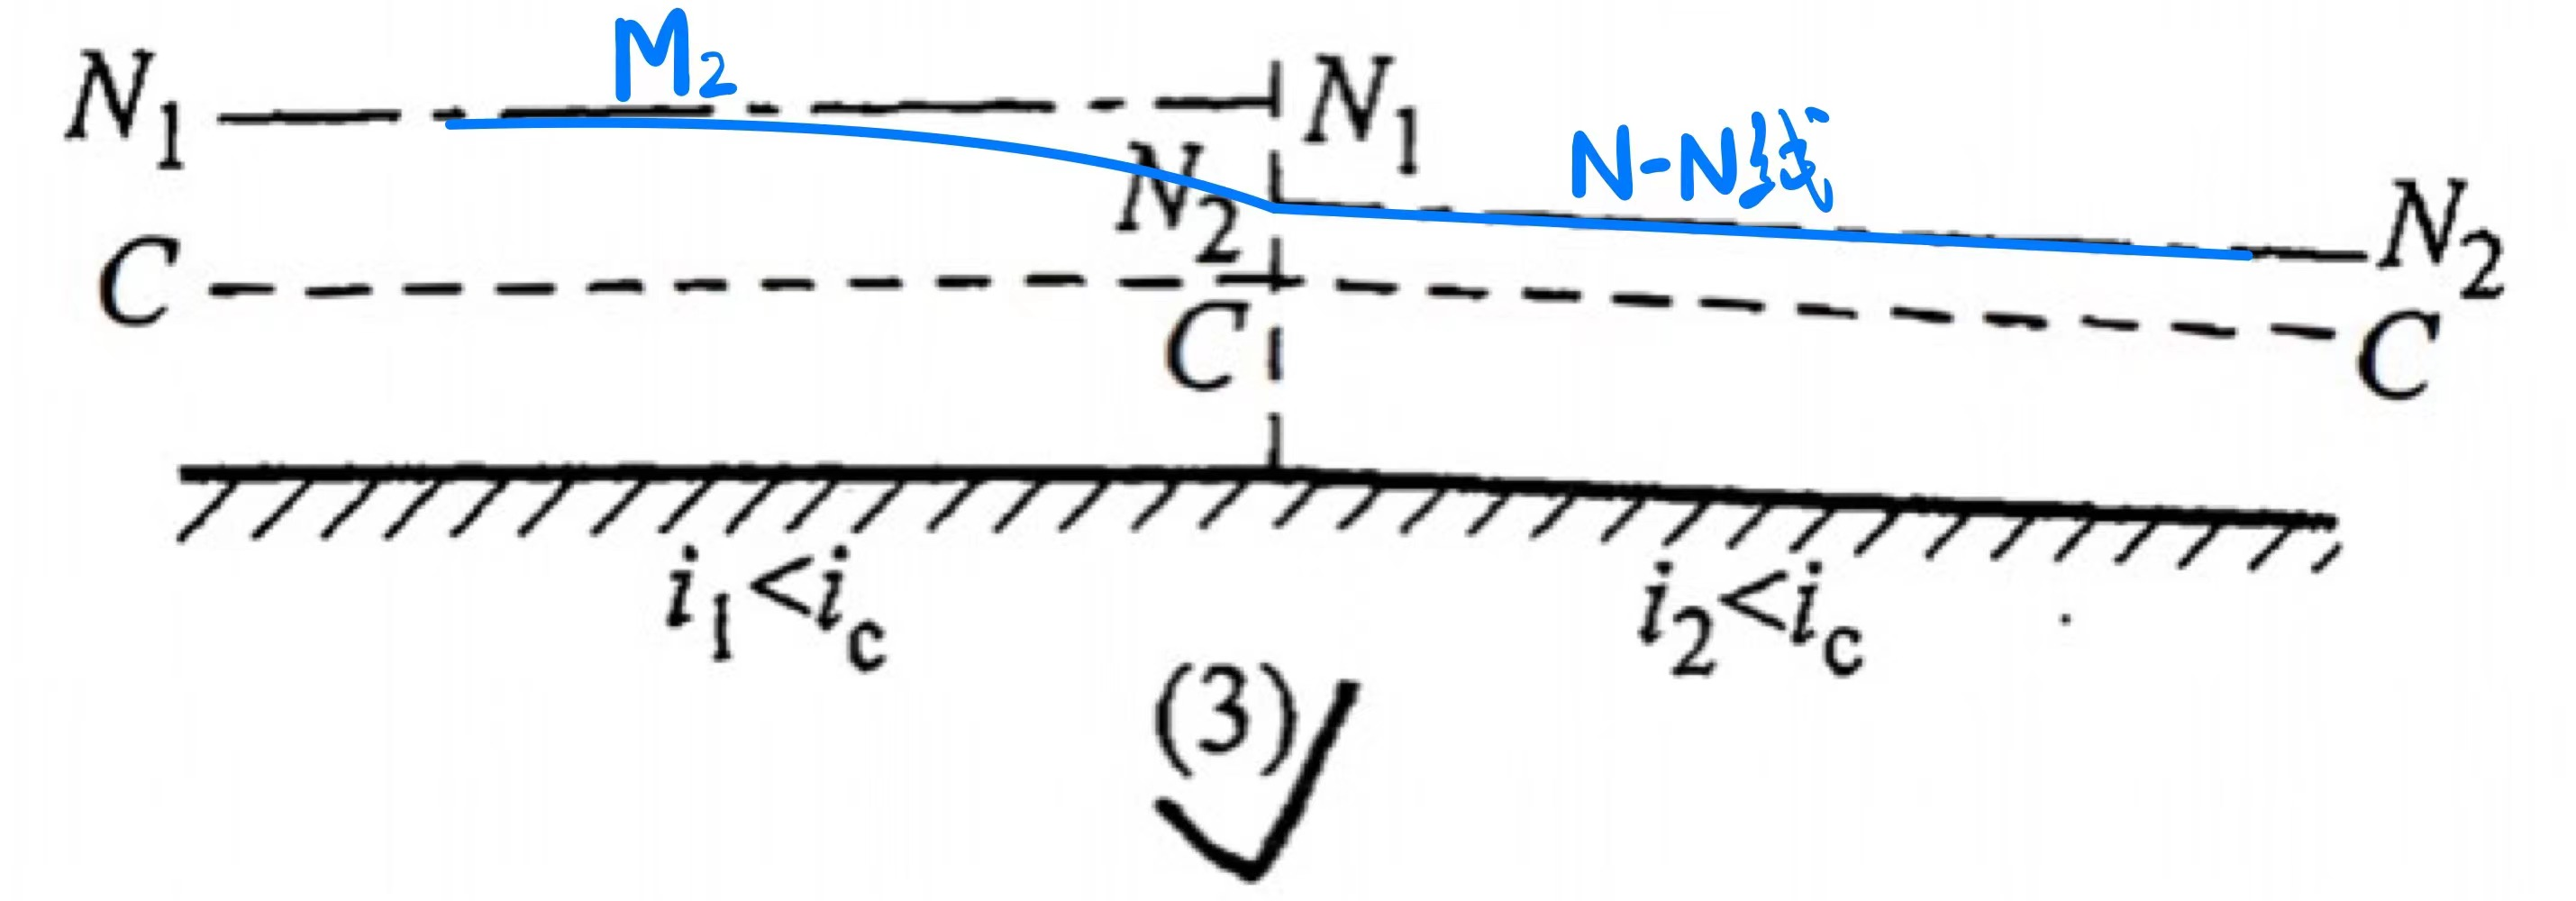
\includegraphics[width=0.80\textwidth]{./assets/1-3.jpg}}
        \subfigure[(4)水面曲线]{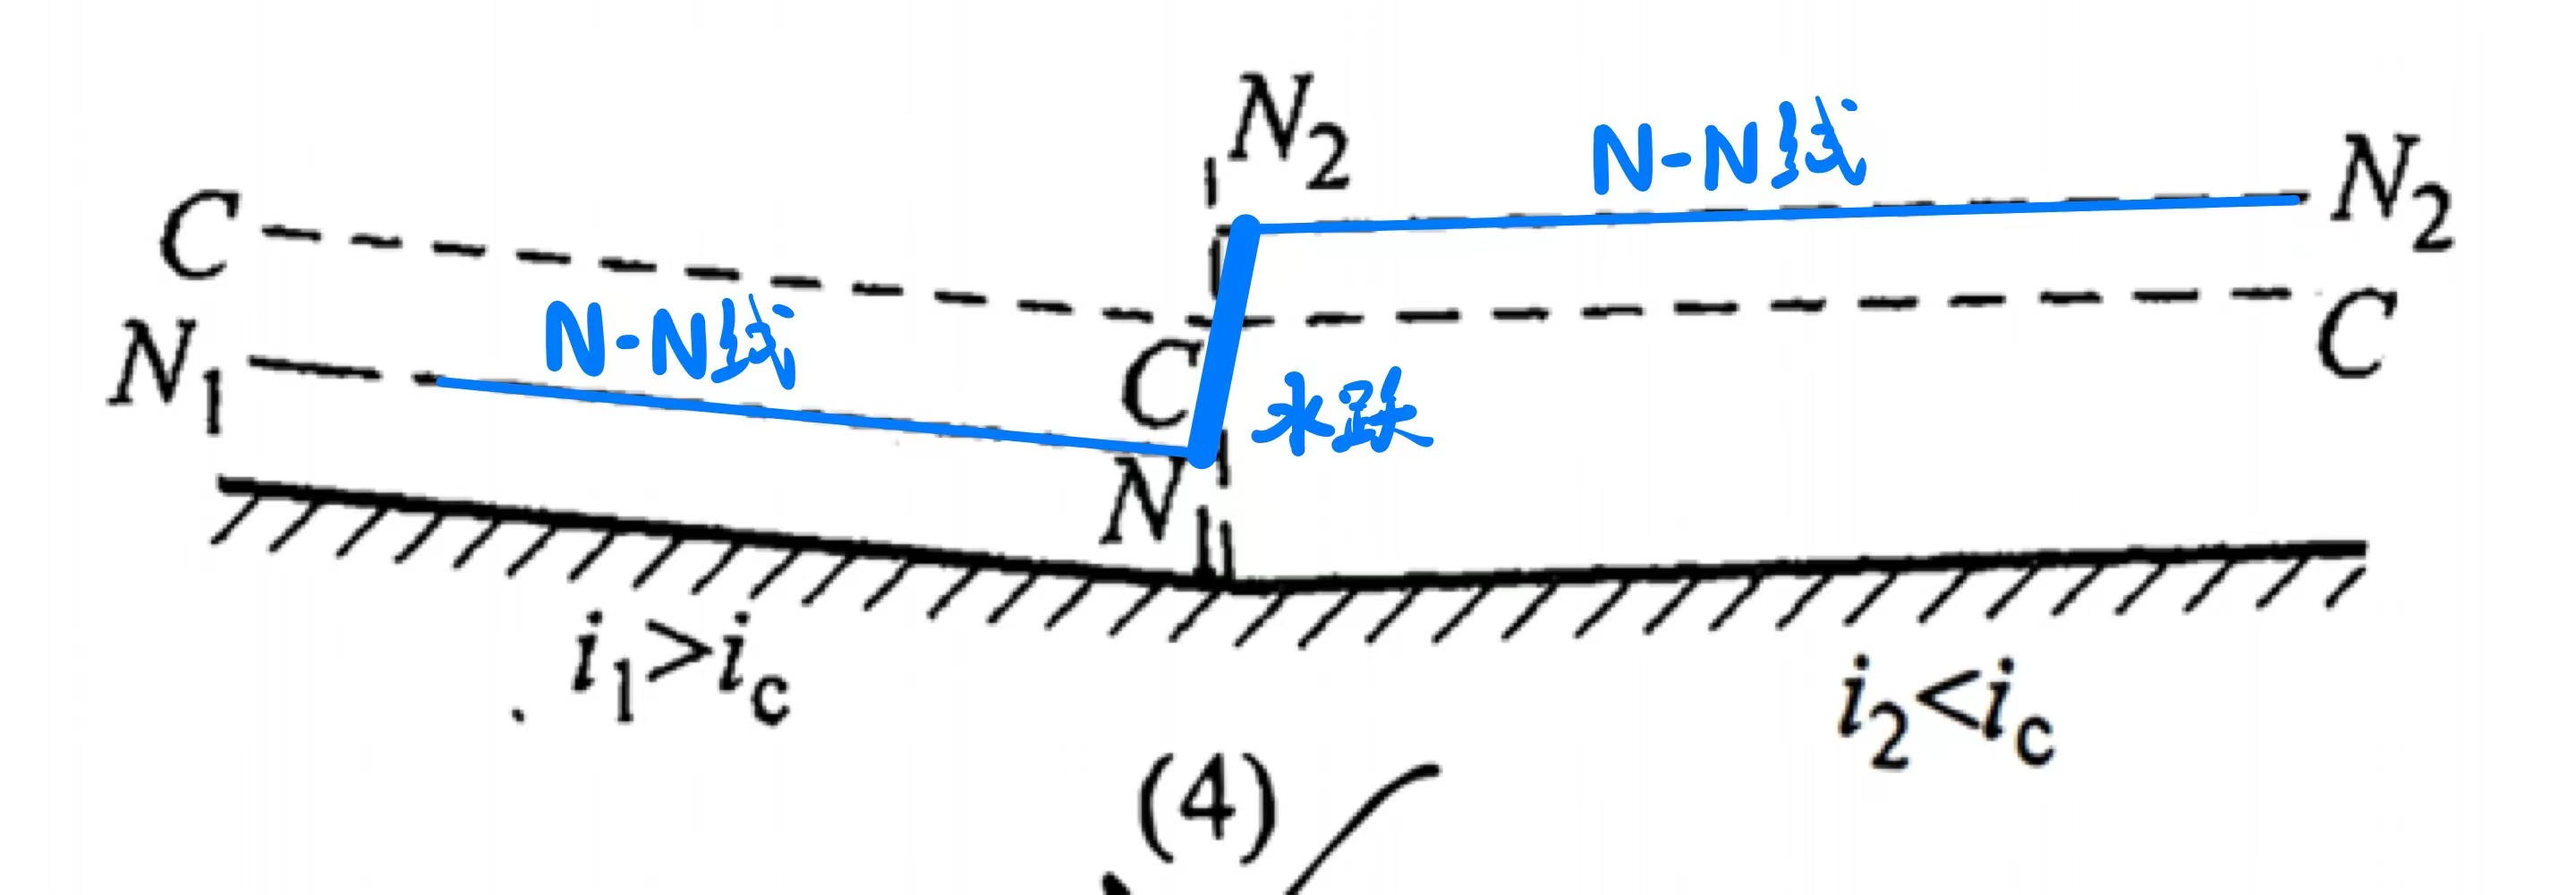
\includegraphics[width=0.80\textwidth]{./assets/1-4.jpg}}
        \caption{题1解答}
        \end{figure}

    \section{}

        i1坡为缓坡。在桥段正常水深略微提高。随后过渡到陡坡i2。
        因此，该部分的水面曲线为$M_1 -> M_2 -> S_2$。

        可以将i3坡视为正常水深无穷高的坡面，因此从i2坡到i3坡会发生短促的淹没水跃。

        随后，在i2坡，水面曲线会在临界水深附近波动，呈$H_2$、$H_3$交替状。
        由于能量损失，波动的波长和振幅均会逐渐衰减。

        从i3坡过渡到i4坡会发生水跃。
        根据i3坡长度的不同，在水跃前的水深可能有不同的取值，因此可能发生两种水跃形态。

        最后，在i4坡，水面曲线恢复至正常水深线。

        综上，可能出现的两种水面曲线如图2所示。

        \begin{figure}[htbp]
        \centering
        \subfigure[case 1]{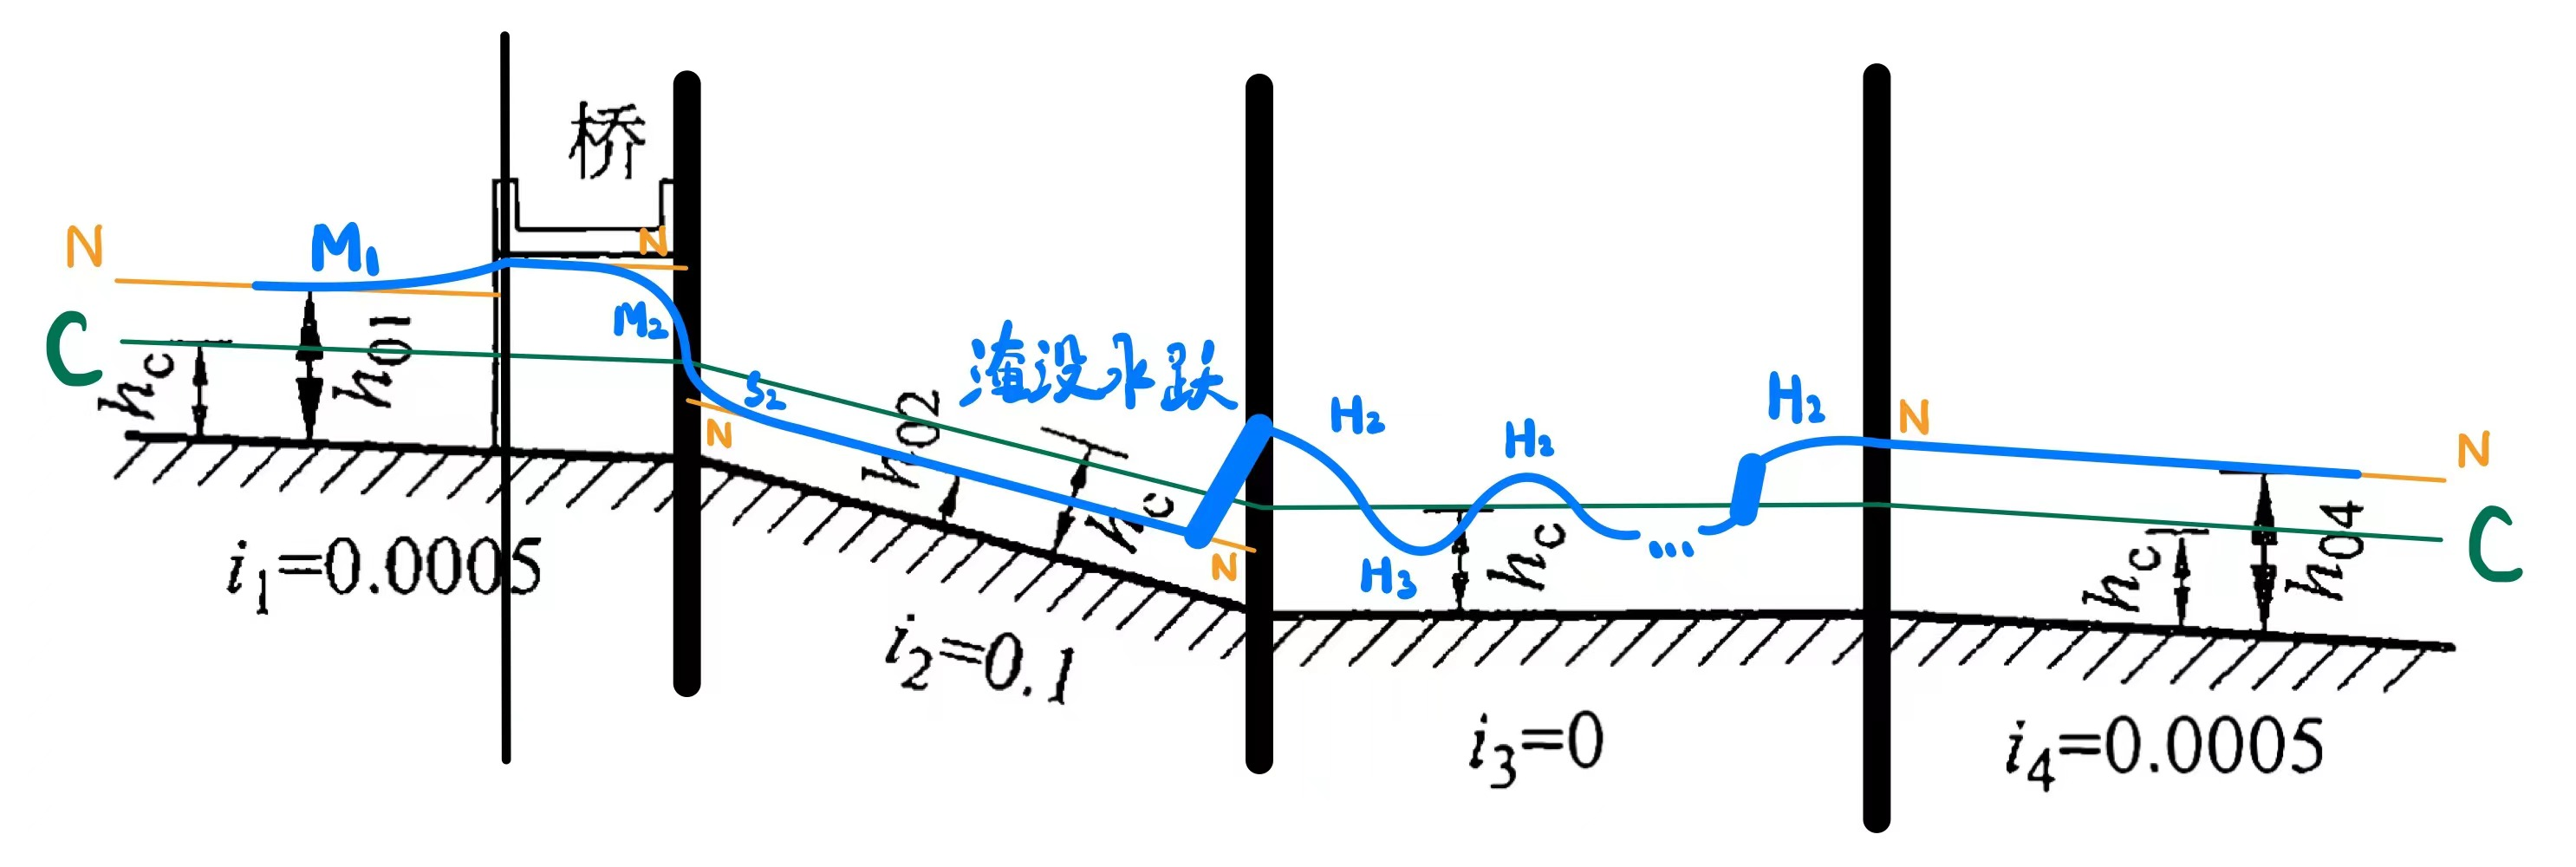
\includegraphics[width=1.00\textwidth]{./assets/2-1.jpg}}
        \subfigure[case 2]{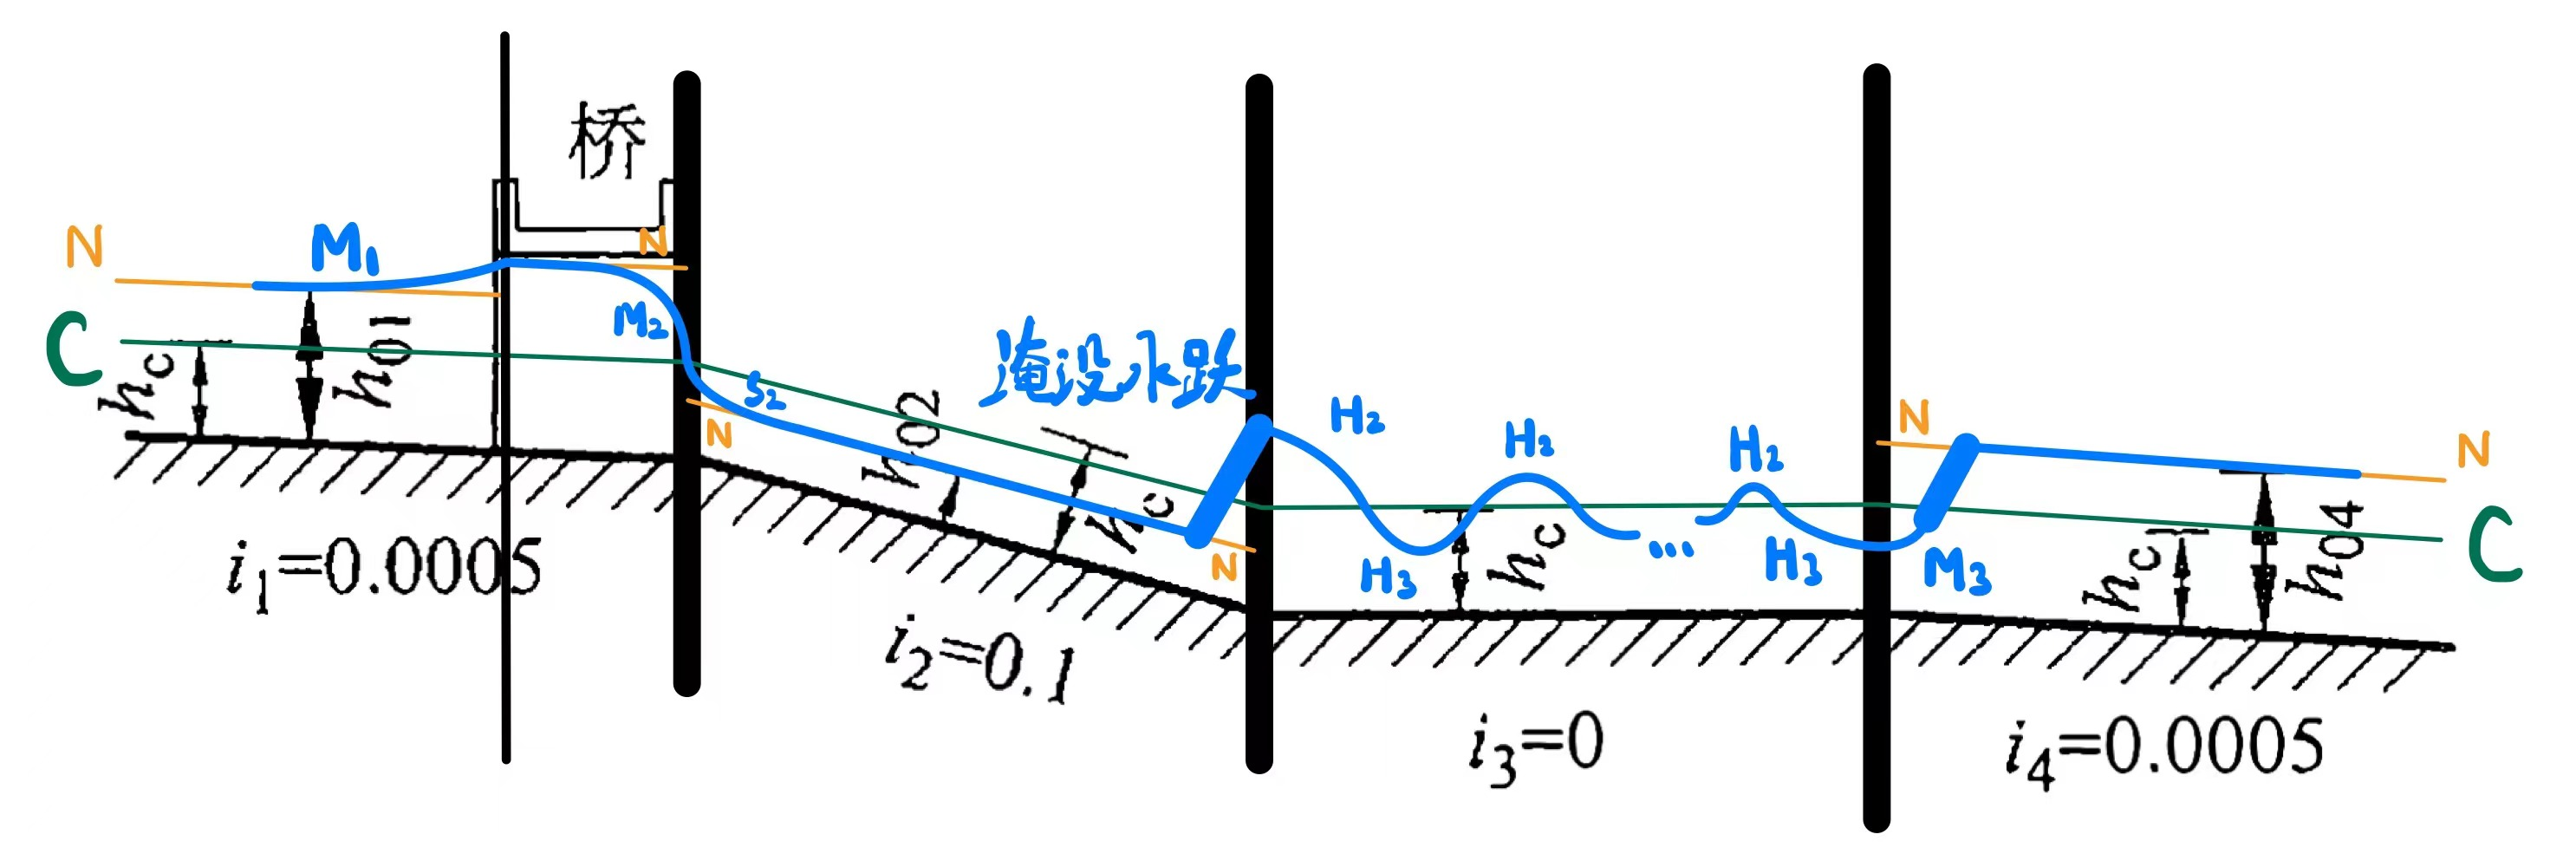
\includegraphics[width=1.00\textwidth]{./assets/2-2.jpg}}
        \caption{题2解答}
        \end{figure}

    \section{}

        \begin{figure}[htbp]
        \centering
        \subfigure{
\includegraphics[width=0.90\textwidth]{./assets/3.png}}
        \caption{题3图}
        \end{figure}

        水跃函数：
        $$J(h) = \frac{\beta_0 Q^2}{g A} + y_c A$$

        其中：$A = h (b + m h)$，$y_c = \frac{h}{6} \frac{3 b + 2 m h}{b + m h}$。

        代入数值，得：
        $$J(h) = \frac{300.866}{h (7 + h)} + \frac{1}{6} h^2 (21 + 2h)$$。

        绘图，结果如图4所示，其中红线为水跃函数曲线。

        \begin{figure}[htbp]
        \centering
        \subfigure{
\includegraphics[width=0.90\textwidth]{./assets/4.png}}
        \caption{水跃函数图像}
        \end{figure}

        已知跃前水深为$h^\prime = 0.8m$。从图中可以看出：共轭水深$h^{\prime\prime} = 3.004 m$。

        当$J(h)$取到最小值时，水深即为临界水深。从图中可以看出：临界水深$h_c = 1.683 m$。

    \section{}

    \subsection{}

    取跃前水深为$h^\prime = 2 m$，临界水深为$h_c = 3 m$。

    注意到上游段的正常水深低于临界水深为陡坡；下游段的正常水深高于临界水深，为缓坡。
    因此在急流向缓流的过度部分会发生水跃。

    对于矩形渠道而言，有：
    $$h_c^3 = \frac{\alpha Q^2}{g b^2} = \frac{\alpha q^2}{g}$$
    $$h^\prime h^{\prime\prime} (h^\prime + h^{\prime\prime}) = \frac{2 \alpha q^2}{g}$$

    于是有关系式：
    $$h^\prime h^{\prime\prime} (h^\prime + h^{\prime\prime}) = 2 h_c^3$$

    代值，计算得：$h^{\prime\prime} = 2 \sqrt{7} - 1 (m) = 4.29 (m)$。

    下游段正常水深$h_t = 5 m > h^{\prime\prime}$，因此水跃类型为淹没水跃。

    水面曲线如图5所示。

    \begin{figure}[htbp]
    \centering
    \subfigure{
\includegraphics[width=0.72\textwidth]{./assets/5.jpg}}
    \caption{水面曲线}
    \end{figure}

    \subsection{}

    下游段正常水深$h_t = 4 m < h^{\prime\prime}$，因此水跃类型为远驱水跃。

    水面曲线如图6所示。

    \begin{figure}[htbp]
    \centering
    \subfigure{
\includegraphics[width=0.72\textwidth]{./assets/6.jpg}}
    \caption{水面曲线}
    \end{figure}

\end{document}
